\section{Theorie}
\label{sec:Theorie}
Das Ziel dieses Versuchs ist es, einen Zusammenhang zwischen Beugungsmuster und dem beugenden Objekt, 
sowie der Aperturfunktion, herzustellen.
Als Beugung wird das Verhalten des Lichts beschrieben, welches von der Geometrichen Optik abweicht, wenn das Licht 
durch Öffnungen eines Schirms oder auf undurchlässige Hindernisse trifft. Dabei müssen die Abmessungen kleiner sein, 
als der Strahlendurchmesser des Lichts. Dieses Phänomen lässt sich nicht mehr durch die Annahme beschreibe, Licht sei ein Teilchen. 
Statdessen wird es, wenn viele Lichtquanten beobachtet werden, gut durch die Annahme, Licht sei eine Welle, beschrieben.

\paragraph{Parallelspalt}
Es gibt generell zwei mögliche Versuchsanordnungen, die Fresnelsche und die Fraunhofersche Lichtbeugung.
Bei der fresnelschen Beugung liegen sowohl die Lichtquelle als auch der Beobachtungspunkt im endlichen Bereich. 
Das hat zur Folge, dass die Lichtstrahlen die an einem Punkt beobachtet werden verschiedene Beugungswinkel haben.
Bei diesem Versuch wird die Fraunhofersche Beugung verwendet, da diese mathematisch einfacher ist als die
Fresnelsche Beugung. Das bedeutet, dass sowohl die Lichtquelle, als auch der Aufpunkt im unendlichen liegen und somit der 
Beugungswinkel für alle Lichtstrahlen eines Beobachtungspunktes gleich ist. 
Die in Z-Richtung einfallende Welle mit der Feldstärke A pro Längeneinheit der Wellenfront wird nun wie folgt beschrieben
\begin{equation}
    \label{eq:1}
    A(z,t) = A_0 exp \left( i(\omega t - \frac{2 \pi z}{\lambda})\right).
\end{equation}
Der verwendete Spalt hat die Breite b und eine Länge die groß gegen b ist. Die Begrenzung des Lichtbündels 
liegt also nur in der X-Koordinate. Der Beobachtungsort wird in einer Entfernung zum Spalt gewählt, die sehr groß 
gegen die Spaltbreite ist.
Durch Kombination des Huygensschen Prinzips der Elementarwellen und dem Interferenzprinzips, entsteht die Annahme, 
der zu beobachtende Schwingungszustand an einem einzelnen Punkt, ist gegeben durch die Überlagerung 
aller Elementarwellen, die zum selben Zeitpunkt im entsprechenden Punkt ankommen.
Abbildung \ref{fig:a} veranschaulicht den Gedanken der Fraunoferschen Beugung schematisch.
\begin{figure}[H]
    \centering
    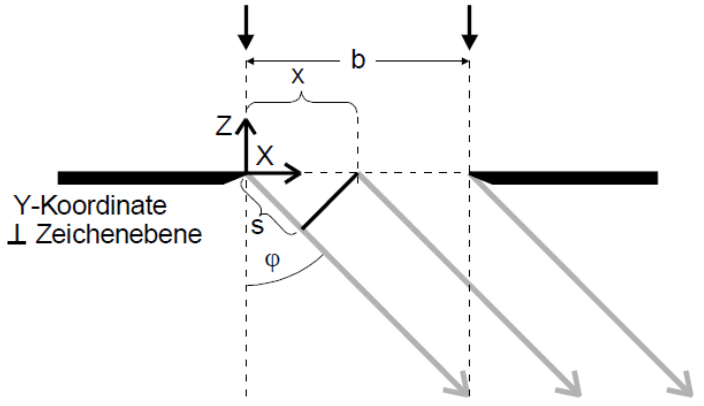
\includegraphics{Spalt.png}
    \caption{Skizze der Fraunhoferschen Beugung \cite{V406}.}
    \label{fig:a}
\end{figure}
Diese einzelnen Elementarwellen sind in Abbildung \ref{fig:a} als Strahlen dargestellt. Weiter ist zu erkennen, dass eben jene 
Elementarwellen die zum selben Zeitpunkt den Beobatungspunkt erreichen und um die Entfernung x im Spalt auseinander liegen, 
sich durch den Wegunterschied s unterscheiden. Da nun von infinitesimale kleinen abständen dx ausgegangen wird, ergibt sich 
für die Amplitund B eine Integration über die gesamte Spaltbreite
\begin{equation}
    \label{eq:2}
    B(z,t,\phi) = A_0 exp\left( i \left( \omega t - \frac{2 \pi z }{\lambda}\right)\right) \int_{0}^{b} exp\left(\frac{2 \pi i x sin \phi}{\lambda}\right) \,dx ,
\end{equation}
woraus sich wiederum nach der Integration und Umformen
\begin{equation}
    \label{eq:3}
    B(z,t,\phi) = A_0 exp\left(i \left(\omega t - \frac{2 \pi z}{\lambda}\right)\right) \cdot exp\left(\frac{\pi i b \, sin \phi}{\lambda}\right) \cdot \frac{\lambda}{\pi b \, sin \phi} sin\left(\frac{\pi b \, sin \phi}{\lambda}\right),
\end{equation}
ergibt.
Die beiden Exponentialfunktionen stellen Phasenfunktionen dar, sind daher für die experimentelle Überprüfung irrelevant.
Dafür ergibt sich dann 
\begin{equation}
    \label{eq:4}
    B(\phi) = A_0 b \frac{sin \nu}{\nu},
\end{equation}
mit $\nu := \frac{\pi b \, sin \phi}{\lambda}$.
Die Funktion ist in Abbildung \ref{fig:b} dargestellt und hat die Nullstellen bei 
\begin{equation}
    \label{eq:5}
    sin \phi_n = \pm n\frac{\lambda}{b}.
\end{equation}
\begin{figure}[H]
    \centering
    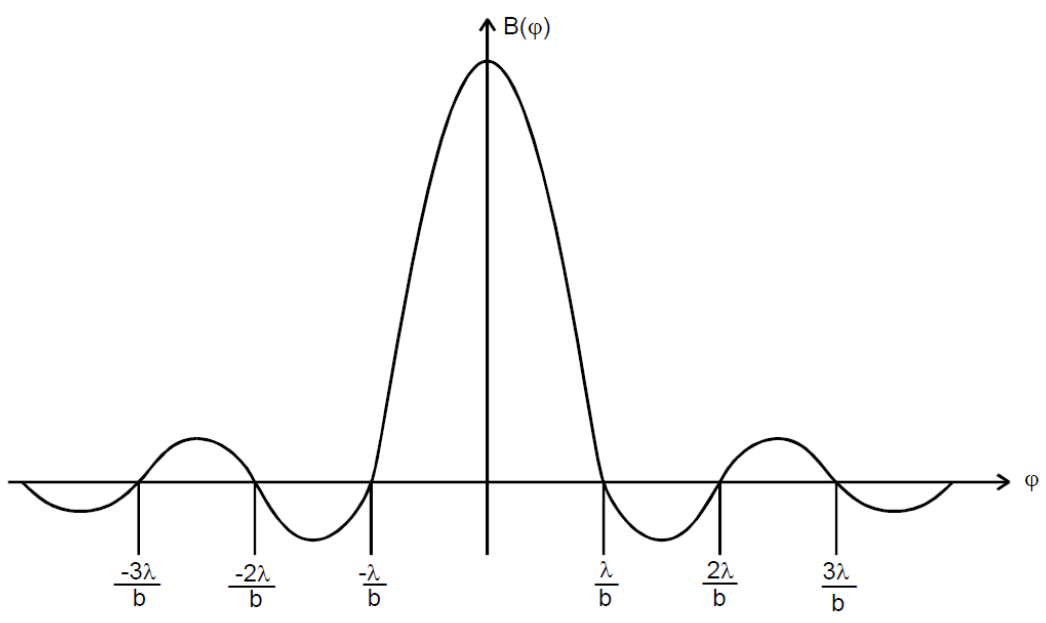
\includegraphics{Funktion.png}
    \caption{Graphische Darstellung der Amplitudenfunktion $B(\phi)$ \cite{V406}.}
    \label{fig:b}
\end{figure}
Die Lichtfrequenz der Lichtwelle $\omega = 10^14$ bis $10^15$ Hz, ist zu hoch für eine unmittelbare Messung, 
weshalb der Mittelwert der Intensität $I(\phi)$ bestimmt wird. Für die Intensität gilt 
\begin{equation}
    \label{eq:6}
    I(\phi) \propto B(\phi)^2 = A_0^2 b^2 \left{\frac{\lambda}{\pi b \, sin \phi}\right}^2 sin^2 \left{\frac{\pi b \, sin \phi}{\lambda}\right}  .
\end{equation}

\paragraph{Beugung am Doppelspalt}
Die Intensitätsverteilung $I(\phi)$ bei einer Beugung am Doppelspalt kann als Überlagerung zweier Beugungen an je 
einem Spalt der Breite b mit Abstand s, wie in Abb \ref{fig:c} dargestellt, betrachtet werden.
Trifft paralleles Licht der Wellenlänge $\lambda$ auf den Doppelspalt, ist die Intensitätsverteilung durch 
\begin{equation}
    \label{eq:7}
    I(\phi) \propto B(\phi)^2 = 4 cos^2\left(\frac{\pi s \, sin \phi}{\lambda}\right) \cdot \left(\frac{\lambda}{\pi b \, sin \phi}\right)^2 \cdot sin^2 \left(\frac{\pi b \, sin \phi}{\lambda}\right)
\end{equation}
gegeben.
\begin{figure}[H]
    \centering
    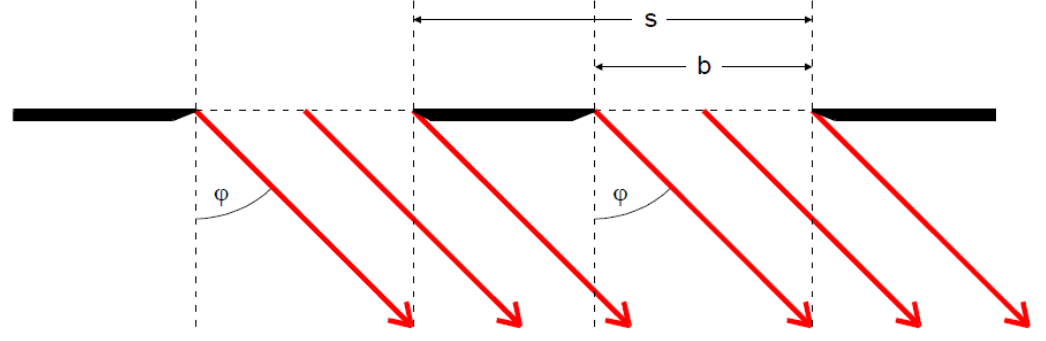
\includegraphics{Doppelspalt.png}
    \caption{Beugung am Doppelspalt \cite{V406}.}
    \label{fig:c}
\end{figure}

\paragraph{Frauenhofersche Beugung und Fourier-Transformation}
Die Fouriertransformierte einer Funktion f(x) ist gegeben durch
\begin{equation}
    \label{eq:8}
    g(\xi) :=  \int_{- \infty}^{+ \infty} f(x) \cdot e^{ix \xi} \,dx.
\end{equation}
Es zeigt sich, dass $B(\phi)$ als Fourier-Transformierte der Aperturfunktion dargestellt werden kann.
In diesem Beispiel ist die Aperturfunktion $f(x) = A_0$ für 0 $\leq$ x $\leq $b und sonst null.
Daraus ergibt sich durch eben jene Fourier-Transformation
\begin{equation}
    \label{eq:9}
    g(\xi) = \frac{2 A_0}{\xi} exp \left(\frac{i \xi b}{2}\right) sin \frac{\xi b}{2},
\end{equation}
mit
\begin{equation}
    \label{eq:10}
    \xi := \frac{2 \pi \, sin \phi}{\lambda}.
\end{equation}
Da die Fourier-Transformierte umkehrbar ist, kann ebenso von der Amplitudenfunktion der Gestalt f(x) auf das brechende 
Objekt geschlossen werden.

